\documentclass[aspectratio=1610,t]{beamer}

% Colors
\usepackage{color}
\definecolor{mainorange}{HTML}{EC811B}
\definecolor{lightgrey}{HTML}{888888}

% Syntax highlighting
\usepackage{minted}
\usepackage{alltt}
\newcommand\hi[1]{{\color{mainorange} \textbf{#1}}}

% Theme
\usetheme[%
	subsectionpage=progressbar,
	numbering=fraction,
	progressbar=foot,
]{metropolis}

% Customization
\setbeamertemplate{section in toc}[sections numbered]
\setbeamerfont{title}{size=\fontsize{30}{30}}
\setbeamerfont{block title}{size=\large}
\newcommand\sep{\textcolor{lightgrey}{\rule{\linewidth}{0.05mm}}}

% Meta
\title{Thread pools and iterators}
\date{\today}
\author{Stefan Schindler (@dns2utf8)}
\institute{Rust Zürichsee, Schweiz CH - @Cosin 2018}

\begin{document}

\pgfdeclareimage[width=\paperwidth]{bg}{background-light.pdf}
\pgfdeclareimage[width=\paperwidth]{bgdark}{background-dark.pdf}

\usebackgroundtemplate{\pgfuseimage{bgdark}}
\maketitle

% ----------------------------------------------------------------- %

\begin{frame}[plain,noframenumbering]
	\frametitle{Inhalt}
	\setcounter{tocdepth}{1}
	\tableofcontents
\end{frame}

% ----------------------------------------------------------------- %

\usebackgroundtemplate{\pgfuseimage{bg}}

{
\usebackgroundtemplate{\pgfuseimage{bgdark}}
\section{Über}
}

%\begin{frame}[fragile]{Timetable}
%  \begin{itemize}
%    \item now => Talk
%    \item 20:00 => Questions
%    \item 20:10 => Happy hacking
%    \item 21:00 => Closing
%    \item tomorrow => ???
%    \item the day after => Parallelize the World!
%  \end{itemize}
%\end{frame}
% timetable


\begin{frame}[fragile]{About:me}
Hallo mein Name ist Stefan und I arbeite an und mit Computern.

Ich organisier
\begin{itemize}
  \item RustFest.eu Paris: 26. \& 27. May mit "impl days" am 28. \& 29. May
  \item Meetups in und um Zürich
  \item Illuminox.ch (in den Schweizer Alpen Juli 2018)
\end{itemize}

Ein paar von meinen Nebenprojekten
\begin{itemize}
  \item rust threadpool
  \item Son of Grid Engine (SGE) interface
  \item run your own infrastructure - DNS, VPN, Web, ...
\end{itemize}
\end{frame}



\begin{frame}[fragile]{Was wir heute lernen werden}

\begin{itemize}
 \item Schleifen
 \item Iteratoren
 \item Verschiedene Ausführungsmodi
 \item Single vs. Multi Threading
 \item Wie man Pools synchronisiert
 \item Wie man linearen Code in parallelen überführt
\end{itemize}

\end{frame}

{
\usebackgroundtemplate{\pgfuseimage{bgdark}}
\section{Schleifen}
}

\begin{frame}[fragile]{Schleifen 0 - Was bisher geschah}
\begin{minted}{C}
const char *data[] = { "Peter Arbeitsloser", ... };

  const int length = sizeof(data) / sizeof(data[0]);
  int index = 0;
kopf:
  if (!(index < length)) {
    goto ende;
  }
  const char *name = data[index];
  printf("%i: %s\n", index, name);
  index += 1;
  goto kopf;
ende:
\end{minted}
\end{frame}

\begin{frame}[fragile]{Schleifen 1 - Was verbessert wurde}
\begin{minted}{C}
const char *data[] = {
    "Peter Arbeitsloser",
    "Sandra Systemadministratorin",
    "Peter Koch",
};

  const int length = sizeof(data) / sizeof(data[0]);

  for (int index = 0; index < length; index++) {
    const char *name = data[index];
    printf("%i: %s\n", index, name);
  }
\end{minted}
\end{frame}

\begin{frame}[fragile]{Schleifen 2}
Die Ausgangslage der folgenden Beispiele:

\begin{minted}{rust}
#[allow(non_upper_case_globals)]
const data: [&str; 3] = [
    "Peter Arbeitsloser",
    "Sandra Systemadministratorin",
    "Peter Koch",
];
\end{minted}
\end{frame}

\begin{frame}[fragile]{Schleifen 3 - While}
\begin{minted}{rust}
    let mut index = 0;
    let length = data.len();
    while index < length {
        println!("{}: {}", index, data[index]);
        index += 1
    }
\end{minted}
\end{frame}

\begin{frame}[fragile]{Schleifen 4 - foreach}
\begin{minted}{rust}
    for name in &data {
        println!("{}", name);
    }
\end{minted}
\end{frame}


{
\usebackgroundtemplate{\pgfuseimage{bgdark}}
\section{Iteratoren}
}

\begin{frame}[fragile]{Trait Iterator}
\begin{minted}{rust}
    pub trait Iterator {
        type Item;
        fn next(&mut self) -> Option<Self::Item>;
    }

    pub enum Option<T> {
        None,
        Some(T),
    }
\end{minted}
\end{frame}

\begin{frame}[fragile]{Iteratoren 0}
\begin{minted}{rust}
    let iterator = data.iter();
    iterator.for_each(|name| {
        println!("{}", name);
    });
\end{minted}

\begin{itemize}
 \item Warum?
 \item Vorteile für
    \begin{itemize}
     \item Programmierer
     \item Compiler
    \end{itemize}
\end{itemize}
\end{frame}



\begin{frame}[fragile]{Iteratoren 1 - Parsen}
\begin{minted}{rust}
struct Person { vorname: String, nachname: String, }
let processed = data
        .iter()
        .map(|name| {
            let mut split = name.split(" ");
let (vorname, nachname) = (split.next(), split.next());
if vorname.is_none() || nachname.is_none() {
    return Err("Konnte namen nicht parsen: Zu wenige Teile")
}
            Ok(Person {
                vorname: vorname.unwrap().into(),
                nachname: nachname.unwrap().into(),
            })
        })
        .collect::<Result<Vec<_>, _>>();
\end{minted}
\end{frame}


\begin{frame}[fragile]{Iteratoren 2 - Parsen}
\begin{minted}{rust}
struct Person { vorname: String, nachname: String, }
let processed = data.iter()
        .map(|name| {
            let mut split = name.split(" ");
let (vorname, nachname) = (split.next(), split.next());
match (vorname, nachname) {
    (Some(vorname), Some(nachname)) => {
        Ok(Person {
            vorname: vorname.into(), nachname: nachname.into(),
        })
    }
    _ => { Err("Konnte namen nicht parsen: Zu wenige Teile") }
}
        })
        .collect::<Result<Vec<_>, _>>();
\end{minted}
\end{frame}



\begin{frame}[fragile]{Iteratoren 3 - Parsen Ergebnis}
\begin{minted}{rust}
processed: Ok(
    [
        Person {
            vorname: "Peter",
            nachname: "Arbeitsloser"
        },
        Person {
            vorname: "Sandra",
            nachname: "Systemadministratorin"
        },
        Person {
            vorname: "Peter",
            nachname: "Koch"
        }
    ]
)
\end{minted}
\end{frame}



{
\usebackgroundtemplate{\pgfuseimage{bgdark}}
\section{Verschiedene Ausführungsmodi}
}

\begin{frame}[fragile]{Programmieren ist ...}
... ein Weg Probleme zu lösen

Beispiele:
\begin{itemize}
  \item Daten kopieren
  \item Audio verbessern
  \item Nachrichten verteilen
  \item Daten speichern
  \item Bilder transformieren
\end{itemize}

Der Schlüssel ist das Problem zu verstehen
\end{frame}

\begin{frame}[fragile]{Single thread - Lineare Ausführung}
Wie erledigen wir mehr als eine Aufgabe gleichzeitig?

\begin{itemize}
  \item Linear wenn die Aufgaben kurz genug sind
  \item Polling
  \item Event getrieben (select/epoll)
  \item Hardware SIMD
\end{itemize}
\end{frame}

\begin{frame}[fragile]{Multi Threading - SMP}
Let's add another level of abstraction
\begin{itemize}
  \item spawn / join: verwalte Listen von JoinHandles
  \item Pools \begin{itemize}
      \item Job Queue (heute das Thema)
      \item Workstealing (rayon)
      \item futures (async / await)
    \end{itemize}
\end{itemize}

Neue Probleme: Synchronisation und Kommunikation

\end{frame}

{
\usebackgroundtemplate{\pgfuseimage{bgdark}}
\section{Implementation}
}

\begin{frame}[fragile]{Send and Sync}
Rusts "pick three" (safety, speed, concurrency)

\begin{minted}{rust}
Trait std::marker::Send
\end{minted}
Typeen können über Thread-Grenzen transferiert werden.

\begin{minted}{rust}
Trait std::marker::Sync
\end{minted}
Typeen können sicher von mehreren Threads referenziert und aufgerufen werden.

\end{frame}

\begin{frame}[fragile]{Crates}
Let's add another level of abstraction
\begin{itemize}
  \item std::thread::{spawn, join}
  \item pools \begin{itemize}
      \item ThreadPool (Job Queue)
      \item FuturesThreadPool (Workstealing)
    \end{itemize}
  \item rayon (Workstealing)
  \item timely dataflow (distributed actor model)
\end{itemize}

Neue Probleme: Synchronisation, Kommunikation und Besitzrecht

\end{frame}

\begin{frame}[fragile]{Channel Beispiel}
\begin{minted}{rust}
use threadpool::ThreadPool; use std::sync::mpsc::channel;

let n_workers = 4; let n_jobs = 8;
let pool = ThreadPool::new(n_workers);

let (tx, rx) = channel();
for _ in 0..n_jobs {
    let tx = tx.clone();
    pool.execute(move || {
        tx.send(1).expect("channel will be there");
    });
}
drop(tx);

assert_eq!(rx.iter().take(n_jobs).fold(0, |a, b| a + b), 8);
\end{minted}
\end{frame}

\begin{frame}[fragile]{Channel Kaskade Beispiel}
\begin{minted}{rust}
let (tx, mut rx) = channel();
tx.send( (0, 0) ).is_ok();
for _ in 0..TEST_TASKS {
    let rx_pre = rx;
    let (tx_chain, rx_chain) = channel();
    rx = rx_chain;

    pool.execute(move || {
        let r = pi_approx_random(VERSUCHE as u64
                                , rand::random::<f64>);
        let b = rx_pre.recv().unwrap();
        tx_chain.send( (b.0 + r.0, b.1 + r.1) ).is_ok();
    });
}
println!("chain.pi: {}", format_pi_approx(rx.recv().unwrap()));
\end{minted}
\end{frame}



{
\usebackgroundtemplate{\pgfuseimage{bgdark}}
\section{Schema: Schleifen zu Iteratoren}
}
\begin{frame}[fragile]{Collect von Channnel - 0}
v\_len speichert wie viele Elemente wir erwarten
\begin{minted}{rust}
  let mut pictures = vec![];

  for _ in 0..v_len {
    if let Some(pi) = rx.recv().unwrap() {
      pictures.push( pi );
    } else {
      // Abbruch wegen einem Fehler
      return;
    }
  }
\end{minted}
\end{frame}

\begin{frame}[fragile]{Collect von Channnel - 1}
Mit foreach brauchen wir die Länge nicht mehr
\begin{minted}{rust}
  let mut pictures = vec![];

  for pi in rx.iter() {
    if let Some(pi) = pi {
      pictures.push( pi );
    } else {
      // Abbruch wegen einem Fehler
      return;
    }
  }
\end{minted}
\end{frame}

\begin{frame}[fragile]{Collect von Channnel - 2}
Mit for\_each brauchen wir die Länge nicht mehr
\begin{minted}{rust}
  let mut pictures = vec![];

  rx.iter().for_each(|pi| {
    if let Some(pi) = pi {
      pictures.push( pi );
    } else {
      // Abbruch wegen einem Fehler
      return;
    }
  });
\end{minted}
\end{frame}

\begin{frame}[fragile]{Collect von Channnel - 3}
\begin{minted}{rust}
  let pictures = rx.iter().map(|pi| {
    if let Some(pi) = pi {
      Ok( pi )
    } else {
      // Abbruch wegen einem Fehler
      Err( () )
    }
  }).collect::<Result<Vec<PictureInfo>, ()>>().unwrap();
\end{minted}
\end{frame}

\begin{frame}[fragile]{Collect von Channnel - 4}
Parallelisiert mit rayon
\begin{minted}{rust}
  let pictures = rx.par_iter().map(|pi| {
    if let Some(pi) = pi {
      Ok( pi )
    } else {
      // Abbruch wegen einem Fehler
      Err( () )
    }
  }).collect::<Result<Vec<PictureInfo>, ()>>().unwrap();
\end{minted}
\end{frame}

%
%{
%\usebackgroundtemplate{\pgfuseimage{bgdark}}
%\section{SGE - Son of Grid Engine}
%}
%\begin{frame}[fragile]{SGE Überblick}
%Entwickelt von SUN
%
%Im Einsatz bei diverse Hochschulen, Universitäten, Firmen und öffentlichen Institutionen ua. (ETH, NASA, ...)
%
%Architektur:
%\begin{itemize}
%    \item Clustermanager läuft auf allen Maschinene
%    \item Benutzer Home auf Cluster Nodes gemountet
%    \item Benutzer schickt ein Shell Skript an den Manager
%\end{itemize}
%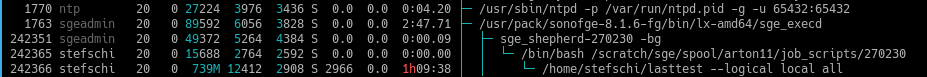
\includegraphics[width=14cm]{Screenshot_SGE_Call.png}
%\end{frame}
%
%\begin{frame}[fragile]{Master Slaves Konzept}
%Nutzen der Umgebungsvariablen \& des Shared Homes
%
%Datei: print.0.sge\_rs
%\begin{verbatim}
%127.0.0.1 ::1 129.132.67.78 fe80::21e:67ff:fe54:9068|arton01
%\end{verbatim}
%
%To the shell now!
%\end{frame}
%
%{
%\usebackgroundtemplate{\pgfuseimage{bgdark}}
%\section{Einige Fallstricke}
%}
%\begin{frame}[fragile]{TcpStream with SGE array jobs}
%X Instanzen erhalten Adressinformationen über die anderen Instanzen
%
%Frage: Wie viele Verbindungen wird jede Instanz öffnen?
%\begin{minted}{rust}
%peer_streams = map.values()
%    .filter(|s| s.is_some())
%    .map(|s| s.unwrap())
%    .map(|(addr, data_port)|
%        TcpStream::connect(
%            SocketAddr::new(addr, data_port)))
%    .filter(|s| s.is_ok())
%    .map(|s| s.unwrap())
%    .collect();
%\end{minted}
%\end{frame}

{
\usebackgroundtemplate{\pgfuseimage{bgdark}}
\section{Fragen}
}

%{
%\usebackgroundtemplate{\pgfuseimage{bgdark}}
%\section{Workshop time}
%}



%\begin{frame}[fragile]{Warum noch eine Sprache?}
%  \begin{itemize}
%    \item Es ist schwer sicheren und korrekten Code zu schreiben.
%    \item Es ist schwierig parallelen Code zu schreiben.
%  \end{itemize}
%
%\begin{minted}{C}
%char *pi = "3.1415926f32";
%while(1) {
%    printf("wie vielte Stelle? ");  err = scanf("%d", &stelle);
%
%    if (err == 0 || errno != 0) {
%      printf("invalid entry\n");    while (getchar() != '\n');
%      continue;
%    }
%
%    printf("Eingabe: %d\n", stelle);
%    printf("Gewünschte Stelle: '%c'\n", pi[stelle]);
%}
%\end{minted}
%\end{frame}





% ----------------------------------------------------------------- %

{
\setbeamertemplate{footline}{}
\pgfdeclareimage[width=\paperwidth]{bg}{background-inverted.pdf}
\usebackgroundtemplate{\pgfuseimage{bg}}
\begin{frame}[standout]
	\begin{centering}
	{\Huge Danke für eure Aufmerksamkeit!}\\
	{\normalsize Stefan Schindler @dns2utf8 }\\
  {\normalsize Happy hacking! Bitte fragt Fragen! }\\
	{\footnotesize Folien \& Beispiele: \url{https://github.com/dns2utf8/thread-pools-and-iterators}}\\
	%{\footnotesize Examples: \url{https://github.com/coredump-ch/intro-to-rust/tree/master/examples}}\\
	\end{centering}
\end{frame}
}

\end{document}
